\documentclass[conference]{IEEEtran}
\usepackage{amsmath,amssymb,booktabs,array,url}
\usepackage{tikz}
\usepackage[hidelinks]{hyperref}
\title{PPO versus DQN for mIoT Random-Access Overload:\\A Reproducible Comparative Study}
\author{\IEEEauthorblockN{DigitalTwinSim Research}
\IEEEauthorblockA{Independent Reproducible Research Artifact}}
\begin{document}
\maketitle

\begin{abstract}
Synchronized massive-IoT (mIoT) arrivals can overload the physical random-access channel (PRACH): devices select the same contention preambles, collide, back off, and retry, potentially sustaining congestion. This paper compares proximal policy optimization (PPO), deep Q-networks (DQN), fixed access class barring (ACB), an adaptive deterministic rule, and no overload control in a browser-executable, 3GPP TR~37.868-inspired simulator. PPO and DQN receive the same 13-variable state, 13-action control set, reward, deterministic action guard, 200 matched training storms, and held-out traffic. In a default 3,000-device storm, both learned controllers outperform fixed ACB, but DQN directly outperforms PPO: DQN obtains 100\% success, zero failures, and 18.6-s 95th-percentile delay, versus 99.8\%, seven failures, and 22.2~s for PPO. Across 30 held-out scenarios, PPO wins none, DQN wins 20, and 10 show mixed trade-offs; PPO's Wilson 95\% win-rate interval is 0--11.4\%. The result rejects an assumed PPO advantage and supports conditional algorithm selection rather than learning-based superiority. Results are synthetic and are neither standards-conformance nor field-performance claims.
\end{abstract}

\begin{IEEEkeywords}
PRACH, mIoT, random access, access class barring, PPO, DQN, overload control.
\end{IEEEkeywords}

\section{Introduction}
Massive machine-type traffic is usually sparse, yet a common alarm, power restoration, coverage recovery, or aligned reporting timer can activate many devices within a short interval. Each eligible device selects a contention preamble in a random access opportunity (RAO). Reuse by multiple devices causes collision in the model; retry traffic may then amplify the initial burst. 3GPP TR~37.868 studies radio-access-network improvements for machine-type-communication overload, including access barring and related controls~\cite{tr37868}.

Prior learning work has optimized ACB with a dueling DQN~\cite{bui2020}, selected less-congested access points with DQN~\cite{bekele2021}, optimized heterogeneous MTC random access~\cite{chen2018}, and resolved collisions through multi-agent DQN~\cite{jadoon2022}. These results motivate a narrower question than ``does reinforcement learning help?'': under the same observations, actions, safety restrictions, traffic, and training budget, does PPO improve upon DQN and transparent deterministic controls?

This paper makes three bounded contributions. First, it defines a reproducible PRACH-only simulator that separates random-access overload from scheduled physical-resource-block allocation. Second, it compares PPO and DQN under a common deterministic capacity/recovery action guard and matched training scenarios. Third, it retains negative results through a predefined win/tie/loss rule. The main finding is that DQN, not PPO, is favored in the present matrix. The contribution is therefore comparative evidence and an inspectable artifact, not a new DQN method or a claim of general network performance.

\section{Relation to Prior Work}
TR~37.868 characterizes access-network overload from large MTC populations and evaluates mechanisms such as access barring~\cite{tr37868}. It motivates the traffic phenomenon and control family used here, but it neither defines a PPO/DQN comparison nor establishes a 5G/6G implementation. We therefore use ``TR~37.868-inspired'' to denote the overload scenario, not conformance.

Bui and Pham jointly tune ACB factor and mean barring time with a dueling DQN, emphasizing energy and delay in LTE mMTC~\cite{bui2020}. Chen and Smith apply deep reinforcement learning to heterogeneous MTC access~\cite{chen2018}. Jadoon \emph{et al.} use shared multi-agent DQN with binary feedback for collision resolution against exponential backoff~\cite{jadoon2022}. Bekele and Choi instead place a DQN decision at the device side to select a less-congested transmission/reception point and report access-delay gains in dense networks~\cite{bekele2021}. These studies establish that DQN-related random-access control is prior art. The present DQN is consequently a comparator, not the claimed invention.

Our differentiator is experimental control. PPO and DQN are placed at the same gNB decision point and receive identical inputs, outputs, guard, reward, training scenario sequence, interaction count, and test seeds. This removes several alternative explanations that arise when comparing results across papers with different objectives or architectures. It also tests PPO despite a plausible reason to expect DQN to fit: the action set is finite and modest. Conversely, PPO could benefit from conservative policy updates and correlated multi-step recovery. The result decides between these hypotheses only within the disclosed model.

\begin{table}[t]
\caption{Positioning relative to selected learning-based RA work.}
\label{tab:prior}
\centering\scriptsize
\setlength{\tabcolsep}{2pt}
\begin{tabular}{p{0.16\columnwidth}p{0.14\columnwidth}p{0.23\columnwidth}p{0.25\columnwidth}}
\toprule
Study & Agent & Main action & Primary comparison\\
\midrule
Bui--Pham~\cite{bui2020} & Dueling DQN & ACB factor/time & Energy--delay ACB\\
Bekele--Choi~\cite{bekele2021} & UE DQN & TRxP selection & 3GPP selection\\
Jadoon \emph{et al.}~\cite{jadoon2022} & Multi-agent DQN & Access decision & Exp. backoff\\
This work & gNB PPO/DQN & ACB/backoff & Matched rules and RL\\
\bottomrule
\end{tabular}
\end{table}

\section{System and Contention Model}
The model contains one gNB and an mIoT population. eMBB and URLLC traffic are outside scope. A scenario specifies storm population $N$, start RAO, activation duration, horizon $T$, contention-preamble count $M$, RAO frequency, retry limit, background arrivals, and seed. Moderate, severe, and extreme profiles activate 1,200 devices over 20 RAOs, 3,000 over 10, and 7,000 over five, respectively. The default uses $M=54$, 10 RAOs/s, ten attempts, and $T=300$.

At RAO $t$, a device eligible under ACB is admitted with probability $p_t$. An admitted device chooses one of $M$ preambles uniformly. A singleton preamble succeeds; an occupancy of two or more collides. A collided device increments its attempt counter and draws a uniform retry backoff from the configured window. An ACB-denied device draws a barring delay and retests later. A device exits through success or retry exhaustion; unfinished devices at the horizon count as failures. The abstraction intentionally omits capture, power ramping, detection error, Random Access Response capacity, and detailed message exchanges.

The controller observes a normalized 13-element state: backlog, new arrivals, collision and success ratios, accumulated failures, mean delay, current admission and backoff, idle-preamble ratio, backlog and arrival trends, oldest-device wait, and near-exhaustion fraction. Thirteen discrete actions provide hold, six absolute control profiles from emergency throttling to fully open access, and independent increments/decrements of admission, barring, and retry backoff.

All learned actions pass through the same deterministic guard. With backlog $B_t$, the admission ceiling is proportional to $0.90M/B_t$. When idle-preamble ratio exceeds 0.65 while collision rate is below 0.25 and backlog remains, a recovery floor proportional to $0.35M/B_t$ prevents indefinite throttling. This guard is not attributed to either learner; guard-only ablation remains future work.

\begin{figure}[t]
\centering
\fbox{\parbox{0.92\columnwidth}{\centering\small
Held-out mIoT arrivals $\rightarrow$ ACB eligibility $\rightarrow$ preamble selection\\
$\downarrow$\\[-2pt]
singleton success $\mid$ collision $\rightarrow$ backoff/retry $\rightarrow$ failure limit\\[2pt]
$\uparrow$ telemetry \hfill gNB rule/PPO/DQN $\rightarrow$ common action guard}}
\caption{PRACH-only evaluation loop. Scheduled data PRBs are outside scope.}
\label{fig:flow}
\end{figure}

\section{Controllers and Learning}
The comparison includes no control ($p_t=1$), fixed ACB, an adaptive rule, DQN, and PPO. Fixed ACB uses $p=0.03$, a two-RAO barring interval, and 12-RAO retry backoff. The adaptive rule estimates admission from $0.55M/B_t$ and increases or decreases timing controls at disclosed collision thresholds.

Both neural controllers use one 24-unit tanh hidden layer. DQN estimates $Q(s,a;\theta)$ and minimizes the temporal-difference error
\begin{equation}
 \left[r_t+\gamma\max_{a'\in\mathcal A_g}Q_{\bar\theta}(s_{t+1},a')-Q_\theta(s_t,a_t)\right]^2,
\end{equation}
where $\mathcal A_g$ is the guard-permitted set. It uses epsilon-greedy exploration, a 12,000-transition replay buffer, batches of 32, and a target-network copy every 120 updates, following the value-learning principle of~\cite{mnih2015}.

PPO has separate 24-unit actor and critic pathways. For probability ratio $\rho_t(\theta)$ and normalized advantage $\hat A_t$, it applies the clipped surrogate
\begin{equation}
L^{\mathrm{clip}}=\mathbb E_t\!\left[\min\!\left(\rho_t\hat A_t,
\mathrm{clip}(\rho_t,1-\epsilon,1+\epsilon)\hat A_t\right)\right],
\end{equation}
with $\epsilon=0.2$, $\gamma=0.97$, learning rate 0.002, and three passes per trajectory~\cite{schulman2017}. Both algorithms train for 200 episodes on the exact same generated storm sequence and receive equal environment interactions; replay makes optimizer-update counts inherently different.

The per-RAO reward credits successful access and post-storm clearance and penalizes collision ratio, retry exhaustion, normalized backlog, waiting pressure, idle preambles while backlog remains, and control magnitude. A terminal penalty covers unfinished devices. Thus blocking all devices cannot obtain a favorable return merely by eliminating collisions.

Table~\ref{tab:config} records the principal reproducibility parameters. The action guard is applied before exploration during training and before greedy selection during evaluation. This ensures that neither learner receives unsafe exploratory privileges and that an apparent algorithm gain cannot be attributed to unequal feasibility constraints.

\begin{table}[t]
\caption{Common learning and evaluation configuration.}
\label{tab:config}
\centering\small
\begin{tabular}{ll}
\toprule
Item & Value\\
\midrule
State/action dimensions & 13 / 13\\
Hidden layer & 24 tanh units\\
Training episodes & 200 matched storms\\
Discount / learning rate & 0.97 / 0.002\\
PPO clip / passes & 0.2 / 3\\
DQN replay / batch & 12,000 / 32\\
Target-copy interval & 120 DQN updates\\
Evaluation & deterministic, masked\\
Default RAOs / preambles & 300 / 54\\
\bottomrule
\end{tabular}
\end{table}

\section{Evaluation Method}
The default held-out seed is 24680; policy initializations use separate disclosed seeds. Deterministic evaluation selects each learner's highest-scoring permitted action. The 30-case matrix crosses three profiles with ten independent traffic seeds per profile. One trained instance of each algorithm is used, so the matrix measures traffic-seed variation, not training-seed uncertainty.

A candidate is non-degrading relative to a comparator when it has no more failures, success is not lower by more than 0.2 percentage points, and 95th-percentile (P95) access delay is within 5\%. A win additionally requires at least a 5\% reduction in failures, collision rate, or P95 delay. Mutual non-degradation without material improvement is a tie; otherwise incomparable KPI directions are ``mixed.'' Wilson intervals summarize observed binary wins but do not describe practical-network confidence.

\section{Artifact Workflow and Auditability}
The artifact executes seven explicit stages. First, it snapshots the storm, PRACH, ACB, rule, and optimizer controls. Second, it generates and freezes the 200 training configurations; both learners receive these configurations in the same order. Third, PPO and DQN train independently with fixed initialization seeds. Fourth, a held-out arrival schedule is generated once per evaluation seed. Fifth, all five controllers process that same schedule using counter-based per-device random values for ACB, preamble choice, and retry backoff. Sixth, controller-independent metrics are computed. Finally, the predefined decision function assigns win, tie, loss, or mixed without replacing or clipping unfavorable values.

The browser exposes two evaluation paths. ``Train and Run'' produces the detailed default table, backlog plot, sampled backlog table, and trace. ``Validation Matrix'' executes three profiles across a configurable number of traffic seeds and exports one CSV row per comparison. The backlog graph's horizontal axis is RAO index and also reports elapsed seconds using the configured RAO rate. The table is important because curve shape alone is ambiguous: a backlog can fall through successful service or through retry exhaustion. Success and failure columns disambiguate those mechanisms.

Randomness is matched where it represents the environment and separated where it represents the algorithms. Traffic and per-device access draws are keyed to the evaluation seed and device/RAO identifiers. PPO and DQN initialization and exploration streams are separate and disclosed. The present matrix holds each learned policy fixed while traffic changes; it therefore avoids retraining on test cases but cannot characterize training-seed variance.

Computational fairness is defined as equal environment interactions, not equal gradient operations. PPO performs three on-policy passes over each trajectory. DQN stores transitions and performs replay minibatches with a target network. Forcing equal gradient counts would erase a defining algorithmic difference, while allowing unequal environment observations would confound sample exposure. The trace consequently records DQN update count and common training episode count. Wall-clock time is implementation- and browser-dependent and is not used as a performance claim.

The common reward can be summarized as
\begin{equation}
r_t = \alpha S_t-\beta C_t-\chi F_t-\delta B_t-\eta I_t-\kappa U_t,
\end{equation}
where $S_t$ is normalized successful access, $C_t$ collision ratio, $F_t$ retry exhaustion, $B_t$ normalized backlog, $I_t$ idle-preamble fraction weighted by backlog, and $U_t$ timing/control cost. A one-time clearance bonus and terminal unfinished-device penalty complete the episode return. The constants are common to both learners; conclusions are conditional on them. Reward sensitivity is a required extension because different operator valuations of energy, delay, and failure could change the ranking.

\section{Results}
Table~\ref{tab:default} reports the default severe storm. No control rapidly exhausts retries, explaining its short apparent delay and early backlog exit despite only 16.48\% success. Such exit is failure, not recovery. Fixed ACB and the adaptive rule reduce overload but leave failures. DQN achieves zero failures and the best delay; PPO also beats fixed ACB under the predefined rule but has seven failures and a 22.2-s P95 delay. Directly, DQN wins over PPO.

\begin{table}[t]
\caption{Default 3,000-device held-out storm.}
\label{tab:default}
\centering\small
\begin{tabular}{lrrrr}
\toprule
Controller & Success & Fail. & Coll. & P95 (s)\\
\midrule
No control & 16.48\% & 2980 & 98.09\% & 1.0\\
Fixed ACB & 94.98\% & 179 & 44.23\% & 21.3\\
Adaptive rule & 92.74\% & 259 & 29.40\% & 24.6\\
DQN & \textbf{100.00\%} & \textbf{0} & 39.41\% & \textbf{18.6}\\
PPO & 99.80\% & 7 & \textbf{30.60\%} & 22.2\\
\bottomrule
\end{tabular}
\end{table}

\begin{figure}[t]
\centering
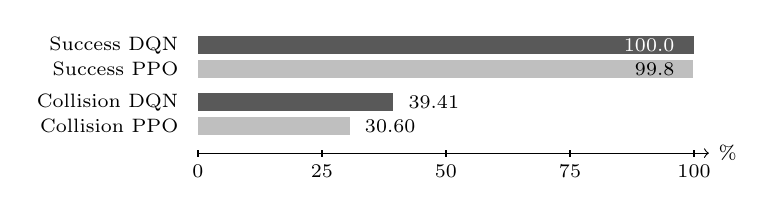
\begin{tikzpicture}[x=0.063cm,y=0.38cm,font=\scriptsize]
  \draw[->] (0,0) -- (103,0) node[right]{\%};
  \foreach \x in {0,25,50,75,100}{\draw (\x,-0.12)--(\x,0.12) node[below=2pt]{\x};}
  \node[anchor=east] at (-2,3.6){Success DQN};
  \node[anchor=east] at (-2,2.8){Success PPO};
  \node[anchor=east] at (-2,1.7){Collision DQN};
  \node[anchor=east] at (-2,0.9){Collision PPO};
  \fill[black!65] (0,3.3) rectangle (100,3.9); \node[anchor=east,text=white] at (98,3.6){100.0};
  \fill[black!25] (0,2.5) rectangle (99.8,3.1); \node[anchor=east] at (98,2.8){99.8};
  \fill[black!65] (0,1.4) rectangle (39.41,2.0); \node[anchor=west] at (40.5,1.7){39.41};
  \fill[black!25] (0,0.6) rectangle (30.60,1.2); \node[anchor=west] at (31.7,0.9){30.60};
\end{tikzpicture}
\caption{Default held-out percentage comparison. DQN: 0 failures and 18.6-s P95 delay; PPO: 7 failures and 22.2-s P95 delay. Other units are stated rather than normalized into the bars.}
\label{fig:comparison}
\end{figure}

Table~\ref{tab:matrix} gives the head-to-head matrix. DQN wins every moderate and severe case. All extreme cases are mixed: neither learner jointly satisfies the other's non-degradation and material-improvement conditions. PPO therefore wins 0/30, DQN wins 20/30, and 10/30 are mixed. The Wilson 95\% interval for PPO's win rate is 0--11.4\%. Against the best deterministic comparator, DQN records 26 wins, one tie, and three losses; PPO records eight wins and 22 losses. These counts favor DQN while also showing that neither learner is uniformly superior to rules.

\begin{table}[t]
\caption{PPO versus DQN over 30 held-out traffic seeds.}
\label{tab:matrix}
\centering\small
\begin{tabular}{lrrrr}
\toprule
Profile & PPO win & DQN win & Tie & Mixed\\
\midrule
Moderate & 0 & 10 & 0 & 0\\
Severe & 0 & 10 & 0 & 0\\
Extreme & 0 & 0 & 0 & 10\\
\midrule
Total & 0 & 20 & 0 & 10\\
\bottomrule
\end{tabular}
\end{table}

The result cautions against choosing PPO because it is newer or policy-based. DQN's replay and discrete value estimation fit this finite action set. PPO may become competitive with continuous controls, more training, or different tuning, but those are hypotheses requiring frozen tests rather than post-result adjustment.

\section{Discussion}
Three observations follow. First, aggregate success alone is insufficient. In the default case PPO reduces collisions relative to DQN (30.60\% versus 39.41\%) yet produces seven failures and materially higher P95 delay. The objective is therefore multi-dimensional: a controller can lower contention by being too restrictive. The terminal-backlog and idle-capacity reward terms reduce this pathology but do not guarantee dominance.

Second, the matrix result is stronger than the favorable result of either learner against fixed ACB. A paper that reported only learned-versus-fixed comparisons could conclude that both methods are effective. The direct matched comparison instead shows that DQN wins all moderate and severe cases. Extreme cases are mixed rather than DQN wins because very concentrated 7,000-device activation creates different collision/delay directions that fail the joint non-degradation rule. Reporting ``mixed'' avoids collapsing incompatible operational trade-offs into a hand-tuned scalar ranking.

Third, the deterministic guard narrows the conclusion. It is operationally useful because it prevents a learned policy from opening far beyond the preamble envelope or remaining closed while resources are idle. However, it also embeds domain knowledge. A guard-only controller might recover much of the learned gain. The next ablation must therefore compare guard-only deterministic selection, unguarded PPO/DQN, and the two guarded learners under the same matrix. Until then, the result supports DQN over PPO \emph{within the shared guard}, not learning over deterministic design in general.

\section{Limitations and Reproducibility}
The simulator is aggregate and synthetic. It is inspired by TR~37.868, an LTE-era MTC study, and does not certify 5G NR or 6G behavior. A single initialization per learner prevents claims about training variance. The common guard may supply much of the benefit; guard-only, unguarded, and Dueling-DQN ablations are required. Fixed parameters were engineering choices rather than exhaustive deterministic optimization. Future validation should add standards-calibrated arrival models, preamble detection and capture, power ramping, response capacity, multiple training seeds, effect sizes, and packet/system-level experiments.

The self-contained browser artifact exposes all scenario, ACB, backoff, PPO, DQN, acceptance, seed, table, trace, and CSV controls. It preserves losses and mixed outcomes. Reproducibility here means that the disclosed computation can be rerun; it does not imply external validity.

\section{Conclusion}
Under matched observations, actions, action guards, training storms, and held-out traffic, DQN outperforms PPO in the default test and in 20 of 30 matrix cases; PPO wins none. Both learning methods can outperform deterministic ACB in selected conditions, but the evidence rejects PPO superiority. The defensible conclusion is conditional selection: for this discrete gNB-side PRACH overload problem, DQN is the stronger learned candidate, while transparent deterministic control remains necessary as a baseline and fallback.

\begin{thebibliography}{8}
\bibitem{tr37868} 3GPP, ``Study on RAN improvements for machine-type communications,'' TR 37.868, ver. 11.0.0, 2011.
\bibitem{bui2020} A.-T. H. Bui and A. T. Pham, ``Deep reinforcement learning-based access class barring for energy-efficient mMTC random access in LTE networks,'' \emph{IEEE Access}, doi: 10.1109/ACCESS.2020.3045811.
\bibitem{bekele2021} Y. Z. Bekele and Y.-J. Choi, ``Random access using deep reinforcement learning in dense mobile networks,'' \emph{Sensors}, vol. 21, no. 9, Art. no. 3210, 2021.
\bibitem{chen2018} Z. Chen and D. B. Smith, ``Heterogeneous machine-type communications in cellular networks: Random access optimization by deep reinforcement learning,'' in \emph{Proc. IEEE ICC}, 2018.
\bibitem{jadoon2022} M. A. Jadoon, A. Pastore, and M. Navarro, ``Collision resolution with deep reinforcement learning for random access in machine-type communication,'' in \emph{Proc. IEEE VTC-Spring}, 2022.
\bibitem{mnih2015} V. Mnih \emph{et al.}, ``Human-level control through deep reinforcement learning,'' \emph{Nature}, vol. 518, pp. 529--533, 2015.
\bibitem{schulman2017} J. Schulman \emph{et al.}, ``Proximal policy optimization algorithms,'' arXiv:1707.06347, 2017.
\bibitem{artifact} DigitalTwinSim Research, ``RANsliceOpt AI v17 PRACH comparative artifact,'' software artifact, 2026.
\end{thebibliography}
\end{document}
